%%%                         Louis-Thibault GAUTHIER                       %%%



\section{Récurrence \& $\sum$, $\prod$ }

\subsection{Rappels}\label{récurrence}


\Rap
{
	Soit $\calP(n)$ une propriété dépendant de $n$ dans  $\NN$. Soit $n_0 \in \NN$. On peut montrer que $\calP(n)$ est vraie pour tout $n$ dans $\NN$, tel que $n\geq n_0$ en montrant successivement :
	\begin{itemize}
		\item \textcolor{gold2}{Initialisation :} $\calP(n_0)$ est vraie.
		\item \textcolor{gold2}{Hérédité :} $\forall n \in \NN, n \geq n_0, \left[\calP(n) \Longrightarrow \calP(n+1)\right]$.
	\end{itemize}
}
Donnons une explication \og heuristique \fg, avec des dominos :
\begin{center}
	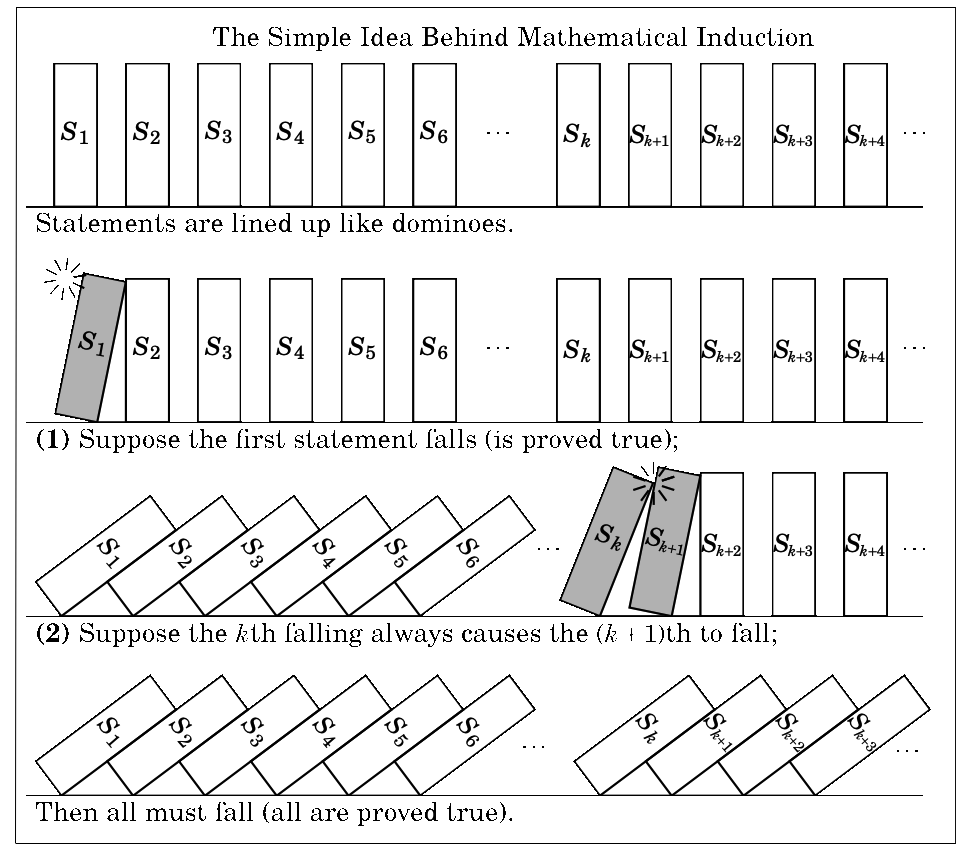
\includegraphics[width=1\linewidth]{../Dessins/induction.png}
\end{center}


\begin{exo}
	Soit $(u_n)_n$ la suite définie par $u_0 := 1$, et :
	\[ 
	\forall n \in \N, \quad u_{n+1} := \ln (1+u_n)
	\]
	Montrer que, pour tout $n$ dans $\N$, $u_n$ est strictement positif.
\end{exo}





\subsection{Sommes $\sum$}


	Soit $(u_k)_{k \in \NN}$ une suite de réels. 
\Def{
	Pour $n \in \NN$, on appelle \textcolor{gold2}{somme des $u_k$, pour $k$ allant de 0 à $n$} , que l'on note : $	\textcolor{gold2}{\displaystyle{\sum_{k=0}^{n}}} u_k$ l'expression \footnotemark : 
	\[ 
		\sum_{k=0}^{n} u_k := u_0 + u_1 + u_2 + \cdots + u_{n-2} + u_{n-1} + u_n
	\]
}
\footnotetext{Qui veut bien dire ce qu'elle veut dire.}


\example
	On a : 
	\[ 
		\sum_{k=0}^{5} k = 0 + 1+2 +3 +4 +5 =  15
	\] 


Il n'est bien sûr, pas obligatoire de sommer en partant de 0. Si $a,b \in \ZZ$, avec $a\leq b$, on généralise la définition précédente pour la somme : $\displaystyle{\sum_{k=a}^{b}} u_k :=  u_a + u_{a+1} + \cdots + u_{b-1} + u_b$ 

\example
	Soit $n \in \NN$, Lorsqu'on parle de $\displaystyle{\sum_{k=-n}^{n}} k$, on parle de :
	\[ 
		\sum_{k=-n}^{n} k =-n - (n-1) - \cdots -1 +0 +1 +\cdots +n \quad  	\mbox{Ce qui est égal ... à } 0 \mbox{ !}%\footnote{Ah bon ?! Pourquoi ?}
	\]



\Prop[(Somme d'une constante)]
{
	\label{SommeC}
	Soit $n \in \NN^*,a,b \in  \ZZ$, tels que $a\leq b$, alors :
	\[ 
		\sum_{k=1}^{n} 1 = \underbrace{1 + \cdots + 1} _{n \mbox{ \tiny 	apparitions de 1}}= n \quad \mbox{et} \quad \sum_{k=a}^{b} 3 = (b-a+1)\times 3
	\]
}
Formule à connaitre par cœur : si $a\leq b \, (\in \ZZ)$, alors $\llbracket a, b \rrbracket$ possède $b-a+1$ éléments !

\vspace{2\baselineskip} 

\Prop[(Sommes géométriques)]
{
	Soit $q \in \RR,n_0,n_1 \in \ZZ$, tels que $n_0 \leq n_1$. Alors\footnotemark:
	\[
		\sum_{k=n_0}^{n_1}q^k = 
		\left\{
			\begin{array}{cll}
			n_1 - n_0 +1 & \mbox{si} & q=1 \\ q^{n_0} \times  \frac{1-q^{n_1-n_0+1}}{1-q} & \mbox{si\footnotemark} & q \neq 1 \end{array}
		\right.
	\]
	En particulier si $n_0 =0$ et $n_1=n$, alors on a plus simplement : 
	\[ 
		\sum_{k=0}^{n} q^k =  
		\left\{ 
			\begin{array}{lll}
				n+1& \mbox{si} & q=1 \\
				\frac{1-q^{n+1}}{1-q} & \mbox{si} & q \neq 1 
			\end{array}
		\right.
	\]
}
\footnotetext[\the\numexpr\value{footnote}-1\relax]{Cette formule est atroce à retenir.}


\footnotetext{Voir la proposition \ref{SommeC} sur cette page.}

Je vous recommande grandement de retenir cette formule dans le cas $q\neq 1$ (raison différente de 1) par une phrase :
\begin{center}
	\large{\textcolor{gold2}{\og  premier terme, fois, $\displaystyle{\frac{\mbox{1 moins raison}^{\mbox{puissance nombre de termes}}}{\mbox{sur, 1 moins raison}}}$ \fg}}
\end{center}



\Rem[Attention aux parenthèses !]
{
	Il ne faut pas confondre $\displaystyle{\sum_{k=0}^{n}}  (k+1)$ avec $\left( \displaystyle{\sum_{k=0}^{n}} k \right) +1$. Pensez-y lorsque vous écrirez un \og $+$ \fg, dans une somme $\Sigma$, par exemple, l'expression sans parenthèses suivante peut être ambiguë.:
	\[ 
		\sum_{k=0}^{n} k +1
	\]
}

\Exo{
	Démontrer par récurrence que :
	\[ 
		\forall n \in \NN, \quad \sum_{k=0}^{n} k = \frac{n(n+1)}{2}
	\]
	En déduire la valeur, pour $n \in \NN^*$, de $\displaystyle{\sum_{k=0}^{n+1}} k$, de  $\displaystyle{\sum_{k=0}^{n-1}} k$, et de  $\displaystyle{\sum_{k=0}^{n^2}} k$
}



\Prop[Linéarité de la somme]
{
	Soit $(u_k)_{k \in \llbracket 0,n\rrbracket},(v_k)_{k \in \llbracket 0,n\rrbracket}$ deux familles de réels. Soit $\lambda,\mu \in \RR \footnotemark$. Alors :
	\[ 
		\sum_{k=0}^{n} \lambda u_k + \mu v_k = \lambda \sum_{k=0}^{n} 	u_k + \mu \sum_{k=0}^{n} v_k
	\]
}
\footnotetext{Autrement dit, qui ne dépendent pas de $k$.}


	Soit $n\in \NN^*$, on a alors :
	\[ 
		\textcolor{gold2}{\sum_{k=1}^{n} k\left(2 - \frac{1}{k}\right)} = 	\sum_{k=1}^{n} 2k - 1 = 2\sum_{k=1}^{n} k - \sum_{k=1}^{n} 1 = n(n+1) - n = n^2 +n - n = \textcolor{gold2}{n^2}
	\]


\Exo{
	Soit $n \in \NN^*$,  et $\alpha \in \RR$, exprimer en fonction de $n$ et de $\alpha$ : \\
	$\displaystyle{\sum_{k=1}^{n}} k\left(\alpha +\frac{4}{k}\right)$
}


\end{document}

\subsection{Changement d'indice $\sum$}


\Prop{[Énoncé théorique]
	Soit $p\in \N^*$.\\
	Une expression à l'aide du symbole $\Sigma$ n'est pas unique. Le changement d'indice usuel est la translation  $k \to k+p$ :
	\[ 
	\sum_{k=1}^{n} a_k = \sum_{k=1+p}^{n+p} a_{k-p}
	\]
}

\example[Pratique]
	Soit $n \in \N,n \geq 2$. Calculer sans utiliser la linéarité de la somme :
	\[ 
	\sum_{k=2}^{n} \left( k - 1 \right)
	\]



\subsection{Produits $\prod$}


\Def{
	Soit $(u_k)_{k \in \N}$ une suite de réels. Soit $n\in \N$. De même que pour les sommes : $\sum$, on appelle \textcolor{gold}{produit des $u_k$, pour $k$ allant de $0$ à $n$}, et note : $\displaystyle{\prod_{k=0}^{n}} u_k$ l'expression :
	
	\[ 
	\textcolor{gold2}{\prod_{k=0}^{n} u_k } := u_0 \times u_1 \times u_2  \times \cdots \times u_{n-2} \times u_{n-1} \times u_n
	\]
}

\Def{[La factorielle]
	Soit $n \in \N^*$. On définit $\textcolor{gold}{n!}$, qui se prononce \og \textcolor{gold}{$n$ factorielle}  ou \textcolor{gold}{factorielle de $n$} \fg, par :
	
	\[ 
	n! := \prod_{k=1}^n k = 1 \times 2 \times 3 \times \cdots \times (n-1) \times n
	\]
	
	Par exemple : $4! := 1 \times 2 \times 3 \times 4 = 24$. On pose par convention : \textcolor{gold}{0! := 1}.
}

\Exo{
	Déterminer $3!$.
}

\Exo{
	Soit $n \in \N^*$. Donner les valeurs de :
	\[ 
	\frac{(n+1)!}{n!} = \qquad  \qquad  \frac{(n+1)!}{(n+2)!}= \qquad  \qquad n\times (n-1)! =
	\]

\Rem{
	Comme souvent, il faut bien mettre des parenthèses lorsque nécessaire : $n + 1!$ n'a pas la même signification que $(n+1)!$.
}


\subsection{Télescopages}


\Prop{[Énoncé théorique]
	Soit $(u_k)_{k \in \N}$ une suite de réels. Soit $n\in \N$. Si la suite  $(a_k)_{k \in \N}$  vérifie : 
	\[ 
	\forall k \in \N, \quad a_k = u_{k+1} - u_k
	\]
	
	Alors la somme :
	\[ 
	\sum_{k=0}^{n} a_k = 	u_{n+1} - u_0
	\]
	
	Bien sûr, comme dans la sous-section \og récurrence \fg, page \pageref{récurrence}, ceci se généralise si la relation est seulement vraie à partir d'un entier $n_0$ au lieu de 0 : Si 	$\forall k \in \N, k\geq n_0,  a_k = u_{k+1} - u_k$, alors $\sum_{k=n_0}^{n} a_k = 	u_{n+1} - u_{n_0}$.
}

\example[Pratique]
	Soit $n \in \N^*$, calculer :
	\[ 
	\sum_{k=1}^{n} \left( \frac{1}{k} - \frac{1}{k+1} \right)
	\]
}



\Prop{[Énoncé théorique]
	Soit $(u_k)_{k \in \N}$ une suite de réels non nuls. Soit $n\in \N$. Si la suite  $(a_k)_{k \in \N}$  vérifie : 
	\[ 
	\forall k \in \N, \quad a_k = \frac{u_{k+1}}{u_k} 
	\]
	
	Alors le produit :
	\[ 
	\prod_{k=0}^{n} a_k = 	\frac{u_{n+1}}{u_0} 
	\]
	
	Bien sûr, comme dans la sous-section \og récurrence \fg, page \pageref{récurrence}, ceci se généralise si la relation est seulement vraie à partir d'un entier $n_0$ au lieu de 0 : Si \\
	$\forall k \in \N, k\geq n_0,  a_k = \frac{u_{k+1}}{u_k} $, alors $\prod_{k=n_0}^{n} a_k = 	\frac{u_{n+1}}{u_{n_0}} $.
}

\example[Pratique]
	Soit $n \in \N^*$, calculer, sans passer par les factorielles :
	\[ 
	\prod_{k=1}^{n} \frac{k+1}{k} 
	\]
}


%%%                         Louis-Thibault GAUTHIER                       %%%